\documentclass[1p]{elsarticle_modified}
%\bibliographystyle{elsarticle-num}

%\usepackage[colorlinks]{hyperref}
%\usepackage{abbrmath_seonhwa} %\Abb, \Ascr, \Acal ,\Abf, \Afrak
\usepackage{amsfonts}
\usepackage{amssymb}
\usepackage{amsmath}
\usepackage{amsthm}
\usepackage{scalefnt}
\usepackage{amsbsy}
\usepackage{kotex}
\usepackage{caption}
\usepackage{subfig}
\usepackage{color}
\usepackage{graphicx}
\usepackage{xcolor} %% white, black, red, green, blue, cyan, magenta, yellow
\usepackage{float}
\usepackage{setspace}
\usepackage{hyperref}

\usepackage{tikz}
\usetikzlibrary{arrows}

\usepackage{multirow}
\usepackage{array} % fixed length table
\usepackage{hhline}

%%%%%%%%%%%%%%%%%%%%%
\makeatletter
\renewcommand*\env@matrix[1][\arraystretch]{%
	\edef\arraystretch{#1}%
	\hskip -\arraycolsep
	\let\@ifnextchar\new@ifnextchar
	\array{*\c@MaxMatrixCols c}}
\makeatother %https://tex.stackexchange.com/questions/14071/how-can-i-increase-the-line-spacing-in-a-matrix
%%%%%%%%%%%%%%%

\usepackage[normalem]{ulem}

\newcommand{\msout}[1]{\ifmmode\text{\sout{\ensuremath{#1}}}\else\sout{#1}\fi}
%SOURCE: \msout is \stkout macro in https://tex.stackexchange.com/questions/20609/strikeout-in-math-mode

\newcommand{\cancel}[1]{
	\ifmmode
	{\color{red}\msout{#1}}
	\else
	{\color{red}\sout{#1}}
	\fi
}

\newcommand{\add}[1]{
	{\color{blue}\uwave{#1}}
}

\newcommand{\replace}[2]{
	\ifmmode
	{\color{red}\msout{#1}}{\color{blue}\uwave{#2}}
	\else
	{\color{red}\sout{#1}}{\color{blue}\uwave{#2}}
	\fi
}

\newcommand{\Sol}{\mathcal{S}} %segment
\newcommand{\D}{D} %diagram
\newcommand{\A}{\mathcal{A}} %arc


%%%%%%%%%%%%%%%%%%%%%%%%%%%%%5 test

\def\sl{\operatorname{\textup{SL}}(2,\Cbb)}
\def\psl{\operatorname{\textup{PSL}}(2,\Cbb)}
\def\quan{\mkern 1mu \triangleright \mkern 1mu}

\theoremstyle{definition}
\newtheorem{thm}{Theorem}[section]
\newtheorem{prop}[thm]{Proposition}
\newtheorem{lem}[thm]{Lemma}
\newtheorem{ques}[thm]{Question}
\newtheorem{cor}[thm]{Corollary}
\newtheorem{defn}[thm]{Definition}
\newtheorem{exam}[thm]{Example}
\newtheorem{rmk}[thm]{Remark}
\newtheorem{alg}[thm]{Algorithm}

\newcommand{\I}{\sqrt{-1}}
\begin{document}

%\begin{frontmatter}
%
%\title{Boundary parabolic representations of knots up to 8 crossings}
%
%%% Group authors per affiliation:
%\author{Yunhi Cho} 
%\address{Department of Mathematics, University of Seoul, Seoul, Korea}
%\ead{yhcho@uos.ac.kr}
%
%
%\author{Seonhwa Kim} %\fnref{s_kim}}
%\address{Center for Geometry and Physics, Institute for Basic Science, Pohang, 37673, Korea}
%\ead{ryeona17@ibs.re.kr}
%
%\author{Hyuk Kim}
%\address{Department of Mathematical Sciences, Seoul National University, Seoul 08826, Korea}
%\ead{hyukkim@snu.ac.kr}
%
%\author{Seokbeom Yoon}
%\address{Department of Mathematical Sciences, Seoul National University, Seoul, 08826,  Korea}
%\ead{sbyoon15@snu.ac.kr}
%
%\begin{abstract}
%We find all boundary parabolic representation of knots up to 8 crossings.
%
%\end{abstract}
%\begin{keyword}
%    \MSC[2010] 57M25 
%\end{keyword}
%
%\end{frontmatter}

%\linenumbers
%\tableofcontents
%
\newcommand\colored[1]{\textcolor{white}{\rule[-0.35ex]{0.8em}{1.4ex}}\kern-0.8em\color{red} #1}%
%\newcommand\colored[1]{\textcolor{white}{ #1}\kern-2.17ex	\textcolor{white}{ #1}\kern-1.81ex	\textcolor{white}{ #1}\kern-2.15ex\color{red}#1	}

{\Large $\underline{12n_{0325}~(K12n_{0325})}$}

\setlength{\tabcolsep}{10pt}
\renewcommand{\arraystretch}{1.6}
\vspace{1cm}\begin{tabular}{m{100pt}>{\centering\arraybackslash}m{274pt}}
\multirow{5}{120pt}{
	\centering
	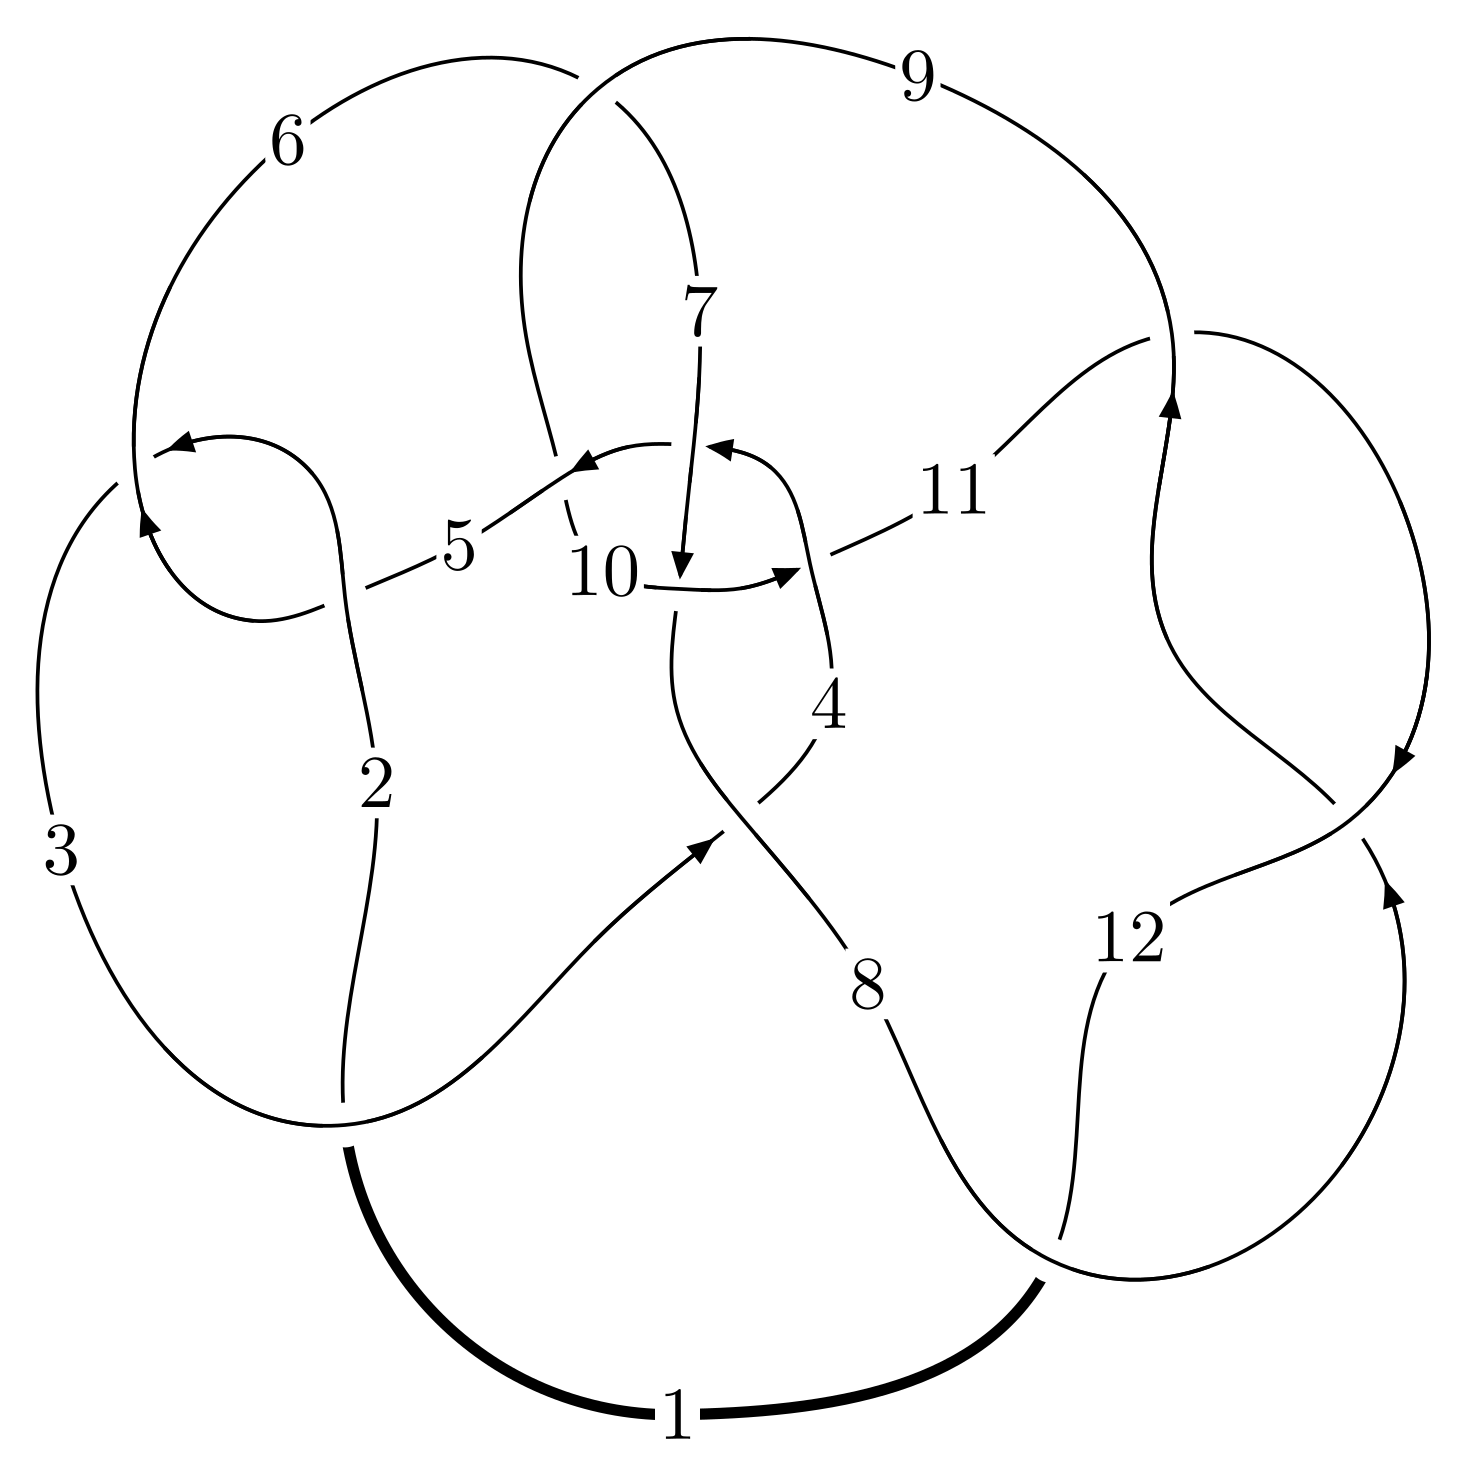
\includegraphics[width=112pt]{../../../GIT/diagram.site/Diagrams/png/2414_12n_0325.png}\\
\ \ \ A knot diagram\footnotemark}&
\allowdisplaybreaks
\textbf{Linearized knot diagam} \\
\cline{2-2}
 &
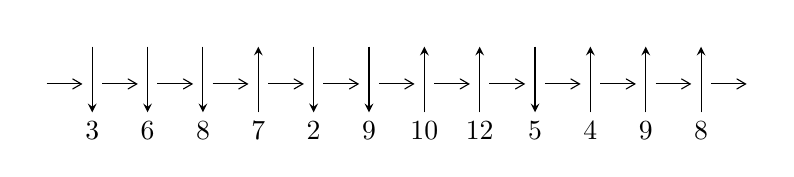
\begin{tikzpicture}[x=20pt, y=17pt]
	% nodes
	\node (C0) at (0, 0) {};
	\node (C1) at (1, 0) {};
	\node (C1U) at (1, +1) {};
	\node (C1D) at (1, -1) {3};

	\node (C2) at (2, 0) {};
	\node (C2U) at (2, +1) {};
	\node (C2D) at (2, -1) {6};

	\node (C3) at (3, 0) {};
	\node (C3U) at (3, +1) {};
	\node (C3D) at (3, -1) {8};

	\node (C4) at (4, 0) {};
	\node (C4U) at (4, +1) {};
	\node (C4D) at (4, -1) {7};

	\node (C5) at (5, 0) {};
	\node (C5U) at (5, +1) {};
	\node (C5D) at (5, -1) {2};

	\node (C6) at (6, 0) {};
	\node (C6U) at (6, +1) {};
	\node (C6D) at (6, -1) {9};

	\node (C7) at (7, 0) {};
	\node (C7U) at (7, +1) {};
	\node (C7D) at (7, -1) {10};

	\node (C8) at (8, 0) {};
	\node (C8U) at (8, +1) {};
	\node (C8D) at (8, -1) {12};

	\node (C9) at (9, 0) {};
	\node (C9U) at (9, +1) {};
	\node (C9D) at (9, -1) {5};

	\node (C10) at (10, 0) {};
	\node (C10U) at (10, +1) {};
	\node (C10D) at (10, -1) {4};

	\node (C11) at (11, 0) {};
	\node (C11U) at (11, +1) {};
	\node (C11D) at (11, -1) {9};

	\node (C12) at (12, 0) {};
	\node (C12U) at (12, +1) {};
	\node (C12D) at (12, -1) {8};
	\node (C13) at (13, 0) {};

	% arrows
	\draw[->,>={angle 60}]
	(C0) edge (C1) (C1) edge (C2) (C2) edge (C3) (C3) edge (C4) (C4) edge (C5) (C5) edge (C6) (C6) edge (C7) (C7) edge (C8) (C8) edge (C9) (C9) edge (C10) (C10) edge (C11) (C11) edge (C12) (C12) edge (C13) ;	\draw[->,>=stealth]
	(C1U) edge (C1D) (C2U) edge (C2D) (C3U) edge (C3D) (C4D) edge (C4U) (C5U) edge (C5D) (C6U) edge (C6D) (C7D) edge (C7U) (C8D) edge (C8U) (C9U) edge (C9D) (C10D) edge (C10U) (C11D) edge (C11U) (C12D) edge (C12U) ;
	\end{tikzpicture} \\
\hhline{~~} \\& 
\textbf{Solving Sequence} \\ \cline{2-2} 
 &
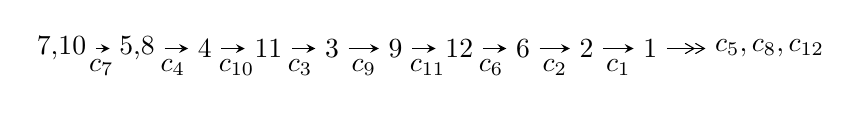
\begin{tikzpicture}[x=23pt, y=7pt]
	% node
	\node (A0) at (-1/8, 0) {7,10};
	\node (A1) at (17/16, 0) {5,8};
	\node (A2) at (17/8, 0) {4};
	\node (A3) at (25/8, 0) {11};
	\node (A4) at (33/8, 0) {3};
	\node (A5) at (41/8, 0) {9};
	\node (A6) at (49/8, 0) {12};
	\node (A7) at (57/8, 0) {6};
	\node (A8) at (65/8, 0) {2};
	\node (A9) at (73/8, 0) {1};
	\node (C1) at (1/2, -1) {$c_{7}$};
	\node (C2) at (13/8, -1) {$c_{4}$};
	\node (C3) at (21/8, -1) {$c_{10}$};
	\node (C4) at (29/8, -1) {$c_{3}$};
	\node (C5) at (37/8, -1) {$c_{9}$};
	\node (C6) at (45/8, -1) {$c_{11}$};
	\node (C7) at (53/8, -1) {$c_{6}$};
	\node (C8) at (61/8, -1) {$c_{2}$};
	\node (C9) at (69/8, -1) {$c_{1}$};
	\node (A10) at (11, 0) {$c_{5},c_{8},c_{12}$};

	% edge
	\draw[->,>=stealth]	
	(A0) edge (A1) (A1) edge (A2) (A2) edge (A3) (A3) edge (A4) (A4) edge (A5) (A5) edge (A6) (A6) edge (A7) (A7) edge (A8) (A8) edge (A9) ;
	\draw[->>,>={angle 60}]	
	(A9) edge (A10);
\end{tikzpicture} \\ 

\end{tabular} \\

\footnotetext{
The image of knot diagram is generated by the software ``\textbf{Draw programme}" developed by Andrew Bartholomew(\url{http://www.layer8.co.uk/maths/draw/index.htm\#Running-draw}), where we modified some parts for our purpose(\url{https://github.com/CATsTAILs/LinksPainter}).
}\phantom \\ \newline 
\centering \textbf{Ideals for irreducible components\footnotemark of $X_{\text{par}}$} 
 
\begin{align*}
I^u_{1}&=\langle 
-5.71883\times10^{322} u^{80}+5.13115\times10^{321} u^{79}+\cdots+1.73962\times10^{324} b+1.35587\times10^{324},\\
\phantom{I^u_{1}}&\phantom{= \langle  }1.38428\times10^{323} u^{80}-6.17270\times10^{322} u^{79}+\cdots+3.47923\times10^{324} a+5.96157\times10^{323},\\
\phantom{I^u_{1}}&\phantom{= \langle  }u^{81}-5 u^{79}+\cdots-56 u+16\rangle \\
I^u_{2}&=\langle 
-6.30190\times10^{15} u^{20}-5.04731\times10^{15} u^{19}+\cdots+9.71732\times10^{16} b-1.02982\times10^{17},\\
\phantom{I^u_{2}}&\phantom{= \langle  }-1.87469\times10^{17} u^{20}-1.88197\times10^{17} u^{19}+\cdots+2.04064\times10^{18} a-8.68955\times10^{18},\\
\phantom{I^u_{2}}&\phantom{= \langle  }u^{21}+u^{20}+\cdots+82 u+21\rangle \\
\\
I^v_{1}&=\langle 
a,\;2 v^3-7 v^2+5 b+6 v+6,\;v^4-4 v^3+6 v^2- v+1\rangle \\
\end{align*}
\raggedright * 3 irreducible components of $\dim_{\mathbb{C}}=0$, with total 106 representations.\\
\footnotetext{All coefficients of polynomials are rational numbers. But the coefficients are sometimes approximated in decimal forms when there is not enough margin.}
\newpage
\renewcommand{\arraystretch}{1}
\centering \section*{I. $I^u_{1}= \langle -5.72\times10^{322} u^{80}+5.13\times10^{321} u^{79}+\cdots+1.74\times10^{324} b+1.36\times10^{324},\;1.38\times10^{323} u^{80}-6.17\times10^{322} u^{79}+\cdots+3.48\times10^{324} a+5.96\times10^{323},\;u^{81}-5 u^{79}+\cdots-56 u+16 \rangle$}
\flushleft \textbf{(i) Arc colorings}\\
\begin{tabular}{m{7pt} m{180pt} m{7pt} m{180pt} }
\flushright $a_{7}=$&$\begin{pmatrix}1\\0\end{pmatrix}$ \\
\flushright $a_{10}=$&$\begin{pmatrix}0\\u\end{pmatrix}$ \\
\flushright $a_{5}=$&$\begin{pmatrix}-0.0397870 u^{80}+0.0177415 u^{79}+\cdots-7.69291 u-0.171347\\0.0328741 u^{80}-0.00294959 u^{79}+\cdots+2.89987 u-0.779406\end{pmatrix}$ \\
\flushright $a_{8}=$&$\begin{pmatrix}1\\- u^2\end{pmatrix}$ \\
\flushright $a_{4}=$&$\begin{pmatrix}-0.0726610 u^{80}+0.0206911 u^{79}+\cdots-10.5928 u+0.608059\\0.0328741 u^{80}-0.00294959 u^{79}+\cdots+2.89987 u-0.779406\end{pmatrix}$ \\
\flushright $a_{11}=$&$\begin{pmatrix}0.0404471 u^{80}-0.0384726 u^{79}+\cdots+16.7195 u-4.06914\\-0.0462175 u^{80}-0.0248072 u^{79}+\cdots-4.11812 u+1.57122\end{pmatrix}$ \\
\flushright $a_{3}=$&$\begin{pmatrix}0.00600531 u^{80}+0.0734423 u^{79}+\cdots-5.37163 u-0.502405\\0.00663013 u^{80}-0.0144926 u^{79}+\cdots+1.20447 u+0.0646126\end{pmatrix}$ \\
\flushright $a_{9}=$&$\begin{pmatrix}-0.0146977 u^{80}-0.0555582 u^{79}+\cdots+8.39910 u-1.39945\\-0.00892733 u^{80}+0.00772163 u^{79}+\cdots-2.20233 u+1.09846\end{pmatrix}$ \\
\flushright $a_{12}=$&$\begin{pmatrix}0.0411094 u^{80}+0.0343150 u^{79}+\cdots+15.7625 u-0.848914\\-0.0733906 u^{80}-0.0529926 u^{79}+\cdots-5.05653 u+1.28512\end{pmatrix}$ \\
\flushright $a_{6}=$&$\begin{pmatrix}-0.157363 u^{80}-0.0629909 u^{79}+\cdots-10.8730 u+2.42951\\0.0162201 u^{80}+0.00434497 u^{79}+\cdots+1.09822 u-0.123036\end{pmatrix}$ \\
\flushright $a_{2}=$&$\begin{pmatrix}-0.0932583 u^{80}-0.0524637 u^{79}+\cdots-11.7756 u+1.50276\\0.0585649 u^{80}+0.0311349 u^{79}+\cdots+3.73976 u-1.21412\end{pmatrix}$ \\
\flushright $a_{1}=$&$\begin{pmatrix}0.0209487 u^{80}+0.00504618 u^{79}+\cdots-11.9699 u+0.112838\\0.0518225 u^{80}+0.0456388 u^{79}+\cdots+3.84524 u-0.655337\end{pmatrix}$\\&\end{tabular}
\flushleft \textbf{(ii) Obstruction class $= -1$}\\~\\
\flushleft \textbf{(iii) Cusp Shapes $= -0.263378 u^{80}-0.100086 u^{79}+\cdots-25.2033 u+11.4620$}\\~\\
\newpage\renewcommand{\arraystretch}{1}
\flushleft \textbf{(iv) u-Polynomials at the component}\newline \\
\begin{tabular}{m{50pt}|m{274pt}}
Crossings & \hspace{64pt}u-Polynomials at each crossing \\
\hline $$\begin{aligned}c_{1}\end{aligned}$$&$\begin{aligned}
&u^{81}+24 u^{80}+\cdots+53 u+1
\end{aligned}$\\
\hline $$\begin{aligned}c_{2},c_{5}\end{aligned}$$&$\begin{aligned}
&u^{81}+2 u^{80}+\cdots+11 u-1
\end{aligned}$\\
\hline $$\begin{aligned}c_{3}\end{aligned}$$&$\begin{aligned}
&u^{81}- u^{80}+\cdots+2043071 u-89033
\end{aligned}$\\
\hline $$\begin{aligned}c_{4}\end{aligned}$$&$\begin{aligned}
&u^{81}+5 u^{80}+\cdots-6 u+1
\end{aligned}$\\
\hline $$\begin{aligned}c_{6}\end{aligned}$$&$\begin{aligned}
&u^{81}+u^{80}+\cdots-13206 u-919
\end{aligned}$\\
\hline $$\begin{aligned}c_{7}\end{aligned}$$&$\begin{aligned}
&u^{81}-5 u^{79}+\cdots-56 u-16
\end{aligned}$\\
\hline $$\begin{aligned}c_{8},c_{11},c_{12}\end{aligned}$$&$\begin{aligned}
&u^{81}-5 u^{80}+\cdots-12 u-1
\end{aligned}$\\
\hline $$\begin{aligned}c_{9}\end{aligned}$$&$\begin{aligned}
&u^{81}+2 u^{80}+\cdots-7 u-11
\end{aligned}$\\
\hline $$\begin{aligned}c_{10}\end{aligned}$$&$\begin{aligned}
&u^{81}+6 u^{80}+\cdots+26845 u-6217
\end{aligned}$\\
\hline
\end{tabular}\\~\\
\newpage\renewcommand{\arraystretch}{1}
\flushleft \textbf{(v) Riley Polynomials at the component}\newline \\
\begin{tabular}{m{50pt}|m{274pt}}
Crossings & \hspace{64pt}Riley Polynomials at each crossing \\
\hline $$\begin{aligned}c_{1}\end{aligned}$$&$\begin{aligned}
&y^{81}+76 y^{80}+\cdots+2869 y-1
\end{aligned}$\\
\hline $$\begin{aligned}c_{2},c_{5}\end{aligned}$$&$\begin{aligned}
&y^{81}-24 y^{80}+\cdots+53 y-1
\end{aligned}$\\
\hline $$\begin{aligned}c_{3}\end{aligned}$$&$\begin{aligned}
&y^{81}+77 y^{80}+\cdots+1032689479609 y-7926875089
\end{aligned}$\\
\hline $$\begin{aligned}c_{4}\end{aligned}$$&$\begin{aligned}
&y^{81}-9 y^{80}+\cdots-158 y-1
\end{aligned}$\\
\hline $$\begin{aligned}c_{6}\end{aligned}$$&$\begin{aligned}
&y^{81}+43 y^{80}+\cdots+71336262 y-844561
\end{aligned}$\\
\hline $$\begin{aligned}c_{7}\end{aligned}$$&$\begin{aligned}
&y^{81}-10 y^{80}+\cdots-448 y-256
\end{aligned}$\\
\hline $$\begin{aligned}c_{8},c_{11},c_{12}\end{aligned}$$&$\begin{aligned}
&y^{81}+17 y^{80}+\cdots-62 y-1
\end{aligned}$\\
\hline $$\begin{aligned}c_{9}\end{aligned}$$&$\begin{aligned}
&y^{81}+14 y^{80}+\cdots-4549 y-121
\end{aligned}$\\
\hline $$\begin{aligned}c_{10}\end{aligned}$$&$\begin{aligned}
&y^{81}-34 y^{80}+\cdots+684980879 y-38651089
\end{aligned}$\\
\hline
\end{tabular}\\~\\
\newpage\flushleft \textbf{(vi) Complex Volumes and Cusp Shapes}
$$\begin{array}{c|c|c}  
\text{Solutions to }I^u_{1}& \I (\text{vol} + \sqrt{-1}CS) & \text{Cusp shape}\\
 \hline 
\begin{aligned}
u &= -0.864704 + 0.515104 I \\
a &= \phantom{-}0.067355 - 0.956329 I \\
b &= -0.77225 - 1.40002 I\end{aligned}
 & \phantom{-}6.65165 - 2.03331 I & \phantom{-0.000000 } 0 \\ \hline\begin{aligned}
u &= -0.864704 - 0.515104 I \\
a &= \phantom{-}0.067355 + 0.956329 I \\
b &= -0.77225 + 1.40002 I\end{aligned}
 & \phantom{-}6.65165 + 2.03331 I & \phantom{-0.000000 } 0 \\ \hline\begin{aligned}
u &= \phantom{-}0.966443 + 0.409894 I \\
a &= -0.339969 + 0.966882 I \\
b &= \phantom{-}1.22854 + 0.97887 I\end{aligned}
 & \phantom{-}2.72616 + 4.53398 I & \phantom{-0.000000 } 0 \\ \hline\begin{aligned}
u &= \phantom{-}0.966443 - 0.409894 I \\
a &= -0.339969 - 0.966882 I \\
b &= \phantom{-}1.22854 - 0.97887 I\end{aligned}
 & \phantom{-}2.72616 - 4.53398 I & \phantom{-0.000000 } 0 \\ \hline\begin{aligned}
u &= -0.994830 + 0.338608 I \\
a &= \phantom{-}0.006971 + 0.922467 I \\
b &= \phantom{-}0.84421 + 1.40177 I\end{aligned}
 & \phantom{-}6.82770 + 4.65491 I & \phantom{-0.000000 } 0 \\ \hline\begin{aligned}
u &= -0.994830 - 0.338608 I \\
a &= \phantom{-}0.006971 - 0.922467 I \\
b &= \phantom{-}0.84421 - 1.40177 I\end{aligned}
 & \phantom{-}6.82770 - 4.65491 I & \phantom{-0.000000 } 0 \\ \hline\begin{aligned}
u &= \phantom{-}0.995164 + 0.394044 I \\
a &= -0.430835 - 0.371591 I \\
b &= -0.703603 + 0.320798 I\end{aligned}
 & -1.65632 - 4.60349 I & \phantom{-0.000000 } 0 \\ \hline\begin{aligned}
u &= \phantom{-}0.995164 - 0.394044 I \\
a &= -0.430835 + 0.371591 I \\
b &= -0.703603 - 0.320798 I\end{aligned}
 & -1.65632 + 4.60349 I & \phantom{-0.000000 } 0 \\ \hline\begin{aligned}
u &= -0.767333 + 0.520690 I \\
a &= \phantom{-}2.03065 + 0.14534 I \\
b &= -0.606396 + 0.400040 I\end{aligned}
 & \phantom{-}6.34137 - 2.12224 I & \phantom{-0.000000 } 0 \\ \hline\begin{aligned}
u &= -0.767333 - 0.520690 I \\
a &= \phantom{-}2.03065 - 0.14534 I \\
b &= -0.606396 - 0.400040 I\end{aligned}
 & \phantom{-}6.34137 + 2.12224 I & \phantom{-0.000000 } 0\\
 \hline 
 \end{array}$$\newpage$$\begin{array}{c|c|c}  
\text{Solutions to }I^u_{1}& \I (\text{vol} + \sqrt{-1}CS) & \text{Cusp shape}\\
 \hline 
\begin{aligned}
u &= -0.631355 + 0.614749 I \\
a &= -2.17032 - 0.52418 I \\
b &= \phantom{-}0.583634 - 0.494454 I\end{aligned}
 & \phantom{-}5.37211 - 8.58308 I & \phantom{-0.000000 -}0. + 10.97236 I \\ \hline\begin{aligned}
u &= -0.631355 - 0.614749 I \\
a &= -2.17032 + 0.52418 I \\
b &= \phantom{-}0.583634 + 0.494454 I\end{aligned}
 & \phantom{-}5.37211 + 8.58308 I & \phantom{-0.000000 } 0. - 10.97236 I \\ \hline\begin{aligned}
u &= \phantom{-}0.812049 + 0.295790 I \\
a &= -0.080919 - 0.949851 I \\
b &= \phantom{-}1.33248 - 1.24004 I\end{aligned}
 & \phantom{-}7.79780 + 1.80326 I & \phantom{-}6.94176 - 3.29971 I \\ \hline\begin{aligned}
u &= \phantom{-}0.812049 - 0.295790 I \\
a &= -0.080919 + 0.949851 I \\
b &= \phantom{-}1.33248 + 1.24004 I\end{aligned}
 & \phantom{-}7.79780 - 1.80326 I & \phantom{-}6.94176 + 3.29971 I \\ \hline\begin{aligned}
u &= -0.693024 + 0.899959 I \\
a &= \phantom{-}0.453119 - 0.585375 I \\
b &= \phantom{-}0.696516 - 0.250989 I\end{aligned}
 & \phantom{-}0.88281 - 2.11179 I & \phantom{-0.000000 } 0 \\ \hline\begin{aligned}
u &= -0.693024 - 0.899959 I \\
a &= \phantom{-}0.453119 + 0.585375 I \\
b &= \phantom{-}0.696516 + 0.250989 I\end{aligned}
 & \phantom{-}0.88281 + 2.11179 I & \phantom{-0.000000 } 0 \\ \hline\begin{aligned}
u &= \phantom{-}0.709599 + 0.423129 I \\
a &= \phantom{-}0.081228 + 1.049090 I \\
b &= -1.28895 + 1.30848 I\end{aligned}
 & \phantom{-}6.61316 + 8.67249 I & \phantom{-}3.85291 - 8.97147 I \\ \hline\begin{aligned}
u &= \phantom{-}0.709599 - 0.423129 I \\
a &= \phantom{-}0.081228 - 1.049090 I \\
b &= -1.28895 - 1.30848 I\end{aligned}
 & \phantom{-}6.61316 - 8.67249 I & \phantom{-}3.85291 + 8.97147 I \\ \hline\begin{aligned}
u &= \phantom{-}0.938083 + 0.715903 I \\
a &= \phantom{-}0.165581 - 1.167330 I \\
b &= -1.14860 - 1.03079 I\end{aligned}
 & -1.74227 + 9.69257 I & \phantom{-0.000000 } 0 \\ \hline\begin{aligned}
u &= \phantom{-}0.938083 - 0.715903 I \\
a &= \phantom{-}0.165581 + 1.167330 I \\
b &= -1.14860 + 1.03079 I\end{aligned}
 & -1.74227 - 9.69257 I & \phantom{-0.000000 } 0\\
 \hline 
 \end{array}$$\newpage$$\begin{array}{c|c|c}  
\text{Solutions to }I^u_{1}& \I (\text{vol} + \sqrt{-1}CS) & \text{Cusp shape}\\
 \hline 
\begin{aligned}
u &= \phantom{-}0.799263 + 0.166597 I \\
a &= \phantom{-}2.07141 + 1.21207 I \\
b &= -0.806764 - 0.009351 I\end{aligned}
 & \phantom{-}7.11949 - 6.20902 I & \phantom{-}7.94528 + 4.20823 I \\ \hline\begin{aligned}
u &= \phantom{-}0.799263 - 0.166597 I \\
a &= \phantom{-}2.07141 - 1.21207 I \\
b &= -0.806764 + 0.009351 I\end{aligned}
 & \phantom{-}7.11949 + 6.20902 I & \phantom{-}7.94528 - 4.20823 I \\ \hline\begin{aligned}
u &= \phantom{-}0.607583 + 1.032170 I \\
a &= \phantom{-}0.396665 + 1.147560 I \\
b &= \phantom{-}0.370178 + 0.457483 I\end{aligned}
 & -3.53662 + 1.62898 I & \phantom{-0.000000 } 0 \\ \hline\begin{aligned}
u &= \phantom{-}0.607583 - 1.032170 I \\
a &= \phantom{-}0.396665 - 1.147560 I \\
b &= \phantom{-}0.370178 - 0.457483 I\end{aligned}
 & -3.53662 - 1.62898 I & \phantom{-0.000000 } 0 \\ \hline\begin{aligned}
u &= -1.196840 + 0.151285 I \\
a &= \phantom{-}0.484675 + 0.322392 I \\
b &= -0.566636 - 0.008546 I\end{aligned}
 & \phantom{-}2.37854 + 0.00858 I & \phantom{-0.000000 } 0 \\ \hline\begin{aligned}
u &= -1.196840 - 0.151285 I \\
a &= \phantom{-}0.484675 - 0.322392 I \\
b &= -0.566636 + 0.008546 I\end{aligned}
 & \phantom{-}2.37854 - 0.00858 I & \phantom{-0.000000 } 0 \\ \hline\begin{aligned}
u &= -0.437058 + 0.660943 I \\
a &= -0.62890 + 1.51723 I \\
b &= -0.97286 + 1.03700 I\end{aligned}
 & -2.04253 - 6.44979 I & -3.14648 + 2.17088 I \\ \hline\begin{aligned}
u &= -0.437058 - 0.660943 I \\
a &= -0.62890 - 1.51723 I \\
b &= -0.97286 - 1.03700 I\end{aligned}
 & -2.04253 + 6.44979 I & -3.14648 - 2.17088 I \\ \hline\begin{aligned}
u &= \phantom{-}0.706225 + 0.292864 I \\
a &= -2.28510 - 0.86473 I \\
b &= \phantom{-}0.834574 + 0.090973 I\end{aligned}
 & \phantom{-}7.40515 + 0.63413 I & \phantom{-}7.99415 - 1.89608 I \\ \hline\begin{aligned}
u &= \phantom{-}0.706225 - 0.292864 I \\
a &= -2.28510 + 0.86473 I \\
b &= \phantom{-}0.834574 - 0.090973 I\end{aligned}
 & \phantom{-}7.40515 - 0.63413 I & \phantom{-}7.99415 + 1.89608 I\\
 \hline 
 \end{array}$$\newpage$$\begin{array}{c|c|c}  
\text{Solutions to }I^u_{1}& \I (\text{vol} + \sqrt{-1}CS) & \text{Cusp shape}\\
 \hline 
\begin{aligned}
u &= -1.001240 + 0.736005 I \\
a &= \phantom{-}0.256315 - 0.742703 I \\
b &= \phantom{-}1.03551 - 1.10338 I\end{aligned}
 & -0.38191 - 5.09344 I & \phantom{-0.000000 } 0 \\ \hline\begin{aligned}
u &= -1.001240 - 0.736005 I \\
a &= \phantom{-}0.256315 + 0.742703 I \\
b &= \phantom{-}1.03551 + 1.10338 I\end{aligned}
 & -0.38191 + 5.09344 I & \phantom{-0.000000 } 0 \\ \hline\begin{aligned}
u &= \phantom{-}1.151460 + 0.487803 I \\
a &= -0.132708 + 0.482310 I \\
b &= \phantom{-}0.68966 + 1.39312 I\end{aligned}
 & \phantom{-}0.57158 + 4.71464 I & \phantom{-0.000000 } 0 \\ \hline\begin{aligned}
u &= \phantom{-}1.151460 - 0.487803 I \\
a &= -0.132708 - 0.482310 I \\
b &= \phantom{-}0.68966 - 1.39312 I\end{aligned}
 & \phantom{-}0.57158 - 4.71464 I & \phantom{-0.000000 } 0 \\ \hline\begin{aligned}
u &= -0.425288 + 0.605867 I \\
a &= -0.402409 + 0.735878 I \\
b &= -1.41930 + 1.05173 I\end{aligned}
 & -2.12406 - 2.49621 I & -6.63409 + 8.73341 I \\ \hline\begin{aligned}
u &= -0.425288 - 0.605867 I \\
a &= -0.402409 - 0.735878 I \\
b &= -1.41930 - 1.05173 I\end{aligned}
 & -2.12406 + 2.49621 I & -6.63409 - 8.73341 I \\ \hline\begin{aligned}
u &= \phantom{-}0.926610 + 0.858585 I \\
a &= \phantom{-}0.194288 - 1.235310 I \\
b &= -0.596939 - 0.501927 I\end{aligned}
 & -2.98305 + 5.70394 I & \phantom{-0.000000 } 0 \\ \hline\begin{aligned}
u &= \phantom{-}0.926610 - 0.858585 I \\
a &= \phantom{-}0.194288 + 1.235310 I \\
b &= -0.596939 + 0.501927 I\end{aligned}
 & -2.98305 - 5.70394 I & \phantom{-0.000000 } 0 \\ \hline\begin{aligned}
u &= \phantom{-}0.630721 + 0.297315 I \\
a &= \phantom{-}0.044076 - 0.323841 I \\
b &= -1.32512 - 0.80646 I\end{aligned}
 & -1.74333 - 0.96559 I & \phantom{-}2.53517 + 1.89595 I \\ \hline\begin{aligned}
u &= \phantom{-}0.630721 - 0.297315 I \\
a &= \phantom{-}0.044076 + 0.323841 I \\
b &= -1.32512 + 0.80646 I\end{aligned}
 & -1.74333 + 0.96559 I & \phantom{-}2.53517 - 1.89595 I\\
 \hline 
 \end{array}$$\newpage$$\begin{array}{c|c|c}  
\text{Solutions to }I^u_{1}& \I (\text{vol} + \sqrt{-1}CS) & \text{Cusp shape}\\
 \hline 
\begin{aligned}
u &= -1.30677\phantom{ +0.000000I} \\
a &= \phantom{-}0.440104\phantom{ +0.000000I} \\
b &= -0.578903\phantom{ +0.000000I}\end{aligned}
 & \phantom{-}2.39168\phantom{ +0.000000I} & \phantom{-0.000000 } 0 \\ \hline\begin{aligned}
u &= -0.809127 + 1.085380 I \\
a &= \phantom{-}0.348245 - 0.753818 I \\
b &= \phantom{-}1.033020 - 0.878591 I\end{aligned}
 & \phantom{-}0.01437 - 3.34341 I & \phantom{-0.000000 } 0 \\ \hline\begin{aligned}
u &= -0.809127 - 1.085380 I \\
a &= \phantom{-}0.348245 + 0.753818 I \\
b &= \phantom{-}1.033020 + 0.878591 I\end{aligned}
 & \phantom{-}0.01437 + 3.34341 I & \phantom{-0.000000 } 0 \\ \hline\begin{aligned}
u &= -1.343510 + 0.229960 I \\
a &= \phantom{-}0.136679 - 0.733260 I \\
b &= \phantom{-}0.0305346 + 0.0832964 I\end{aligned}
 & \phantom{-}3.06582 - 2.90294 I & \phantom{-0.000000 } 0 \\ \hline\begin{aligned}
u &= -1.343510 - 0.229960 I \\
a &= \phantom{-}0.136679 + 0.733260 I \\
b &= \phantom{-}0.0305346 - 0.0832964 I\end{aligned}
 & \phantom{-}3.06582 + 2.90294 I & \phantom{-0.000000 } 0 \\ \hline\begin{aligned}
u &= -0.742009 + 1.145830 I \\
a &= -0.219888 + 0.773292 I \\
b &= -1.113060 + 0.863158 I\end{aligned}
 & -0.56917 - 7.09177 I & \phantom{-0.000000 } 0 \\ \hline\begin{aligned}
u &= -0.742009 - 1.145830 I \\
a &= -0.219888 - 0.773292 I \\
b &= -1.113060 - 0.863158 I\end{aligned}
 & -0.56917 + 7.09177 I & \phantom{-0.000000 } 0 \\ \hline\begin{aligned}
u &= \phantom{-}0.329952 + 0.525230 I \\
a &= \phantom{-}0.736440 - 0.506654 I \\
b &= -0.702528 - 0.710743 I\end{aligned}
 & -1.71749 - 0.71942 I & -4.34292 + 2.51779 I \\ \hline\begin{aligned}
u &= \phantom{-}0.329952 - 0.525230 I \\
a &= \phantom{-}0.736440 + 0.506654 I \\
b &= -0.702528 + 0.710743 I\end{aligned}
 & -1.71749 + 0.71942 I & -4.34292 - 2.51779 I \\ \hline\begin{aligned}
u &= \phantom{-}0.529505 + 0.274692 I \\
a &= \phantom{-}1.46484 - 0.92641 I \\
b &= -0.980346 - 0.517594 I\end{aligned}
 & -2.36369 - 0.32690 I & -5.66562 - 9.76585 I\\
 \hline 
 \end{array}$$\newpage$$\begin{array}{c|c|c}  
\text{Solutions to }I^u_{1}& \I (\text{vol} + \sqrt{-1}CS) & \text{Cusp shape}\\
 \hline 
\begin{aligned}
u &= \phantom{-}0.529505 - 0.274692 I \\
a &= \phantom{-}1.46484 + 0.92641 I \\
b &= -0.980346 + 0.517594 I\end{aligned}
 & -2.36369 + 0.32690 I & -5.66562 + 9.76585 I \\ \hline\begin{aligned}
u &= -0.244534 + 0.536517 I \\
a &= -0.53817 + 1.53698 I \\
b &= -0.451773 + 1.306960 I\end{aligned}
 & -3.40204 + 1.03279 I & -10.82794 - 0.78219 I \\ \hline\begin{aligned}
u &= -0.244534 - 0.536517 I \\
a &= -0.53817 - 1.53698 I \\
b &= -0.451773 - 1.306960 I\end{aligned}
 & -3.40204 - 1.03279 I & -10.82794 + 0.78219 I \\ \hline\begin{aligned}
u &= \phantom{-}0.96412 + 1.05607 I \\
a &= \phantom{-}0.231870 - 0.803520 I \\
b &= -0.645655 - 0.795469 I\end{aligned}
 & -5.04671 + 3.28136 I & \phantom{-0.000000 } 0 \\ \hline\begin{aligned}
u &= \phantom{-}0.96412 - 1.05607 I \\
a &= \phantom{-}0.231870 + 0.803520 I \\
b &= -0.645655 + 0.795469 I\end{aligned}
 & -5.04671 - 3.28136 I & \phantom{-0.000000 } 0 \\ \hline\begin{aligned}
u &= -0.386461 + 0.412162 I \\
a &= \phantom{-}0.76468 - 1.82667 I \\
b &= \phantom{-}0.797237 - 0.778612 I\end{aligned}
 & \phantom{-}0.25040 - 1.87331 I & \phantom{-}0.34554 + 1.40917 I \\ \hline\begin{aligned}
u &= -0.386461 - 0.412162 I \\
a &= \phantom{-}0.76468 + 1.82667 I \\
b &= \phantom{-}0.797237 + 0.778612 I\end{aligned}
 & \phantom{-}0.25040 + 1.87331 I & \phantom{-}0.34554 - 1.40917 I \\ \hline\begin{aligned}
u &= -0.524498 + 0.044281 I \\
a &= -1.62507 - 3.02956 I \\
b &= \phantom{-}0.330303 + 0.197370 I\end{aligned}
 & -1.24173 + 1.81398 I & \phantom{-}10.77561 - 2.15505 I \\ \hline\begin{aligned}
u &= -0.524498 - 0.044281 I \\
a &= -1.62507 + 3.02956 I \\
b &= \phantom{-}0.330303 - 0.197370 I\end{aligned}
 & -1.24173 - 1.81398 I & \phantom{-}10.77561 + 2.15505 I \\ \hline\begin{aligned}
u &= -1.27771 + 0.86343 I \\
a &= -0.047743 - 1.024450 I \\
b &= \phantom{-}1.120830 - 0.833024 I\end{aligned}
 & \phantom{-}8.49340 - 2.81545 I & \phantom{-0.000000 } 0\\
 \hline 
 \end{array}$$\newpage$$\begin{array}{c|c|c}  
\text{Solutions to }I^u_{1}& \I (\text{vol} + \sqrt{-1}CS) & \text{Cusp shape}\\
 \hline 
\begin{aligned}
u &= -1.27771 - 0.86343 I \\
a &= -0.047743 + 1.024450 I \\
b &= \phantom{-}1.120830 + 0.833024 I\end{aligned}
 & \phantom{-}8.49340 + 2.81545 I & \phantom{-0.000000 } 0 \\ \hline\begin{aligned}
u &= \phantom{-}1.29919 + 0.91454 I \\
a &= -0.029009 + 0.970536 I \\
b &= \phantom{-}1.16686 + 1.06335 I\end{aligned}
 & \phantom{-}8.08845 + 10.56960 I & \phantom{-0.000000 } 0 \\ \hline\begin{aligned}
u &= \phantom{-}1.29919 - 0.91454 I \\
a &= -0.029009 - 0.970536 I \\
b &= \phantom{-}1.16686 - 1.06335 I\end{aligned}
 & \phantom{-}8.08845 - 10.56960 I & \phantom{-0.000000 } 0 \\ \hline\begin{aligned}
u &= -0.110881 + 0.394837 I \\
a &= \phantom{-}1.95199 - 1.20586 I \\
b &= \phantom{-}0.744067 - 0.566714 I\end{aligned}
 & \phantom{-}0.24040 - 1.80693 I & \phantom{-}2.04275 + 2.63185 I \\ \hline\begin{aligned}
u &= -0.110881 - 0.394837 I \\
a &= \phantom{-}1.95199 + 1.20586 I \\
b &= \phantom{-}0.744067 + 0.566714 I\end{aligned}
 & \phantom{-}0.24040 + 1.80693 I & \phantom{-}2.04275 - 2.63185 I \\ \hline\begin{aligned}
u &= \phantom{-}1.08582 + 1.16909 I \\
a &= \phantom{-}0.014716 + 0.711655 I \\
b &= \phantom{-}0.351527 + 0.836307 I\end{aligned}
 & -4.65186 + 4.67041 I & \phantom{-0.000000 } 0 \\ \hline\begin{aligned}
u &= \phantom{-}1.08582 - 1.16909 I \\
a &= \phantom{-}0.014716 - 0.711655 I \\
b &= \phantom{-}0.351527 - 0.836307 I\end{aligned}
 & -4.65186 - 4.67041 I & \phantom{-0.000000 } 0 \\ \hline\begin{aligned}
u &= -1.29087 + 0.98632 I \\
a &= \phantom{-}0.033830 + 0.966217 I \\
b &= -1.121530 + 0.843319 I\end{aligned}
 & \phantom{-}8.31128 - 9.42962 I & \phantom{-0.000000 } 0 \\ \hline\begin{aligned}
u &= -1.29087 - 0.98632 I \\
a &= \phantom{-}0.033830 - 0.966217 I \\
b &= -1.121530 - 0.843319 I\end{aligned}
 & \phantom{-}8.31128 + 9.42962 I & \phantom{-0.000000 } 0 \\ \hline\begin{aligned}
u &= \phantom{-}1.28305 + 1.03050 I \\
a &= -0.017196 - 0.966057 I \\
b &= -1.16141 - 1.06158 I\end{aligned}
 & \phantom{-}6.9973 + 17.3859 I & \phantom{-0.000000 } 0\\
 \hline 
 \end{array}$$\newpage$$\begin{array}{c|c|c}  
\text{Solutions to }I^u_{1}& \I (\text{vol} + \sqrt{-1}CS) & \text{Cusp shape}\\
 \hline 
\begin{aligned}
u &= \phantom{-}1.28305 - 1.03050 I \\
a &= -0.017196 + 0.966057 I \\
b &= -1.16141 + 1.06158 I\end{aligned}
 & \phantom{-}6.9973 - 17.3859 I & \phantom{-0.000000 } 0 \\ \hline\begin{aligned}
u &= \phantom{-}0.137169 + 0.220166 I \\
a &= -3.82003 - 1.10596 I \\
b &= \phantom{-}0.891385 + 0.431882 I\end{aligned}
 & \phantom{-}0.27565 + 2.32917 I & \phantom{-}3.22220 - 5.32820 I \\ \hline\begin{aligned}
u &= \phantom{-}0.137169 - 0.220166 I \\
a &= -3.82003 + 1.10596 I \\
b &= \phantom{-}0.891385 - 0.431882 I\end{aligned}
 & \phantom{-}0.27565 - 2.32917 I & \phantom{-}3.22220 + 5.32820 I \\ \hline\begin{aligned}
u &= -1.17162 + 1.66414 I \\
a &= \phantom{-}0.358589 - 0.091080 I \\
b &= \phantom{-}0.791006 + 0.130196 I\end{aligned}
 & \phantom{-}6.40830 - 5.94458 I & \phantom{-0.000000 } 0 \\ \hline\begin{aligned}
u &= -1.17162 - 1.66414 I \\
a &= \phantom{-}0.358589 + 0.091080 I \\
b &= \phantom{-}0.791006 - 0.130196 I\end{aligned}
 & \phantom{-}6.40830 + 5.94458 I & \phantom{-0.000000 } 0 \\ \hline\begin{aligned}
u &= \phantom{-}0.90423 + 1.87894 I \\
a &= \phantom{-}0.385525 - 0.088992 I \\
b &= \phantom{-}0.503904 - 0.470029 I\end{aligned}
 & \phantom{-}5.85315 - 1.73778 I & \phantom{-0.000000 } 0 \\ \hline\begin{aligned}
u &= \phantom{-}0.90423 - 1.87894 I \\
a &= \phantom{-}0.385525 + 0.088992 I \\
b &= \phantom{-}0.503904 + 0.470029 I\end{aligned}
 & \phantom{-}5.85315 + 1.73778 I & \phantom{-0.000000 } 0 \\ \hline\begin{aligned}
u &= -1.44010 + 1.58883 I \\
a &= -0.276887 + 0.100013 I \\
b &= -0.715602 - 0.117841 I\end{aligned}
 & \phantom{-}6.92752 + 0.05311 I & \phantom{-0.000000 } 0 \\ \hline\begin{aligned}
u &= -1.44010 - 1.58883 I \\
a &= -0.276887 - 0.100013 I \\
b &= -0.715602 + 0.117841 I\end{aligned}
 & \phantom{-}6.92752 - 0.05311 I & \phantom{-0.000000 } 0 \\ \hline\begin{aligned}
u &= \phantom{-}1.23014 + 1.82253 I \\
a &= -0.354642 + 0.037461 I \\
b &= -0.487203 + 0.423434 I\end{aligned}
 & \phantom{-}5.57490 - 8.01859 I & \phantom{-0.000000 } 0\\
 \hline 
 \end{array}$$\newpage$$\begin{array}{c|c|c}  
\text{Solutions to }I^u_{1}& \I (\text{vol} + \sqrt{-1}CS) & \text{Cusp shape}\\
 \hline 
\begin{aligned}
u &= \phantom{-}1.23014 - 1.82253 I \\
a &= -0.354642 - 0.037461 I \\
b &= -0.487203 - 0.423434 I\end{aligned}
 & \phantom{-}5.57490 + 8.01859 I & \phantom{-0.000000 } 0\\
 \hline 
 \end{array}$$\newpage\newpage\renewcommand{\arraystretch}{1}
\centering \section*{II. $I^u_{2}= \langle -6.30\times10^{15} u^{20}-5.05\times10^{15} u^{19}+\cdots+9.72\times10^{16} b-1.03\times10^{17},\;-1.87\times10^{17} u^{20}-1.88\times10^{17} u^{19}+\cdots+2.04\times10^{18} a-8.69\times10^{18},\;u^{21}+u^{20}+\cdots+82 u+21 \rangle$}
\flushleft \textbf{(i) Arc colorings}\\
\begin{tabular}{m{7pt} m{180pt} m{7pt} m{180pt} }
\flushright $a_{7}=$&$\begin{pmatrix}1\\0\end{pmatrix}$ \\
\flushright $a_{10}=$&$\begin{pmatrix}0\\u\end{pmatrix}$ \\
\flushright $a_{5}=$&$\begin{pmatrix}0.0918677 u^{20}+0.0922247 u^{19}+\cdots+10.1330 u+4.25825\\0.0648523 u^{20}+0.0519414 u^{19}+\cdots+5.88126 u+1.05978\end{pmatrix}$ \\
\flushright $a_{8}=$&$\begin{pmatrix}1\\- u^2\end{pmatrix}$ \\
\flushright $a_{4}=$&$\begin{pmatrix}0.0270155 u^{20}+0.0402833 u^{19}+\cdots+4.25169 u+3.19848\\0.0648523 u^{20}+0.0519414 u^{19}+\cdots+5.88126 u+1.05978\end{pmatrix}$ \\
\flushright $a_{11}=$&$\begin{pmatrix}0.0296731 u^{20}-0.00117994 u^{19}+\cdots+0.685337 u-1.65814\\-0.0772922 u^{20}-0.0464391 u^{19}+\cdots-6.97105 u-2.24662\end{pmatrix}$ \\
\flushright $a_{3}=$&$\begin{pmatrix}0.0848197 u^{20}+0.0837459 u^{19}+\cdots+8.47766 u+3.97963\\0.0928914 u^{20}+0.0432223 u^{19}+\cdots+5.91914 u+0.758605\end{pmatrix}$ \\
\flushright $a_{9}=$&$\begin{pmatrix}-0.105108 u^{20}-0.0586467 u^{19}+\cdots-9.56290 u-3.55257\\-0.0574885 u^{20}-0.0110277 u^{19}+\cdots-1.27718 u+0.352191\end{pmatrix}$ \\
\flushright $a_{12}=$&$\begin{pmatrix}0.0605212 u^{20}-0.0278204 u^{19}+\cdots+2.53288 u-1.40578\\-0.103104 u^{20}-0.0661692 u^{19}+\cdots-9.85278 u-3.47866\end{pmatrix}$ \\
\flushright $a_{6}=$&$\begin{pmatrix}0.114510 u^{20}+0.0669967 u^{19}+\cdots+8.10574 u+3.53448\\0.0512777 u^{20}-0.0647731 u^{19}+\cdots-2.39869 u-1.32518\end{pmatrix}$ \\
\flushright $a_{2}=$&$\begin{pmatrix}0.0680487 u^{20}+0.00948640 u^{19}+\cdots+3.03949 u+0.327223\\0.0863649 u^{20}-0.0650135 u^{19}+\cdots-0.705523 u-1.34773\end{pmatrix}$ \\
\flushright $a_{1}=$&$\begin{pmatrix}0.0140821 u^{20}-0.0536105 u^{19}+\cdots-1.34684 u-3.02927\\-0.120235 u^{20}-0.0659225 u^{19}+\cdots-9.13478 u-3.04503\end{pmatrix}$\\&\end{tabular}
\flushleft \textbf{(ii) Obstruction class $= 1$}\\~\\
\flushleft \textbf{(iii) Cusp Shapes $= -\frac{49669659860913382}{97173200599743577} u^{20}-\frac{4115535744999369}{97173200599743577} u^{19}+\cdots-\frac{2760913852914928753}{97173200599743577} u-\frac{1471524814101360942}{97173200599743577}$}\\~\\
\newpage\renewcommand{\arraystretch}{1}
\flushleft \textbf{(iv) u-Polynomials at the component}\newline \\
\begin{tabular}{m{50pt}|m{274pt}}
Crossings & \hspace{64pt}u-Polynomials at each crossing \\
\hline $$\begin{aligned}c_{1}\end{aligned}$$&$\begin{aligned}
&u^{21}-9 u^{20}+\cdots+13 u-1
\end{aligned}$\\
\hline $$\begin{aligned}c_{2}\end{aligned}$$&$\begin{aligned}
&u^{21}+3 u^{20}+\cdots- u-1
\end{aligned}$\\
\hline $$\begin{aligned}c_{3}\end{aligned}$$&$\begin{aligned}
&u^{21}-2 u^{20}+\cdots+8 u-1
\end{aligned}$\\
\hline $$\begin{aligned}c_{4}\end{aligned}$$&$\begin{aligned}
&u^{21}+u^{19}+\cdots+3 u+1
\end{aligned}$\\
\hline $$\begin{aligned}c_{5}\end{aligned}$$&$\begin{aligned}
&u^{21}-3 u^{20}+\cdots- u+1
\end{aligned}$\\
\hline $$\begin{aligned}c_{6}\end{aligned}$$&$\begin{aligned}
&u^{21}-2 u^{20}+\cdots-6 u^2+1
\end{aligned}$\\
\hline $$\begin{aligned}c_{7}\end{aligned}$$&$\begin{aligned}
&u^{21}+u^{20}+\cdots+82 u+21
\end{aligned}$\\
\hline $$\begin{aligned}c_{8}\end{aligned}$$&$\begin{aligned}
&u^{21}+6 u^{20}+\cdots+2 u+1
\end{aligned}$\\
\hline $$\begin{aligned}c_{9}\end{aligned}$$&$\begin{aligned}
&u^{21}-2 u^{19}+\cdots-4 u^2+1
\end{aligned}$\\
\hline $$\begin{aligned}c_{10}\end{aligned}$$&$\begin{aligned}
&u^{21}-4 u^{19}+\cdots-2 u^2+1
\end{aligned}$\\
\hline $$\begin{aligned}c_{11},c_{12}\end{aligned}$$&$\begin{aligned}
&u^{21}-6 u^{20}+\cdots+2 u-1
\end{aligned}$\\
\hline
\end{tabular}\\~\\
\newpage\renewcommand{\arraystretch}{1}
\flushleft \textbf{(v) Riley Polynomials at the component}\newline \\
\begin{tabular}{m{50pt}|m{274pt}}
Crossings & \hspace{64pt}Riley Polynomials at each crossing \\
\hline $$\begin{aligned}c_{1}\end{aligned}$$&$\begin{aligned}
&y^{21}+11 y^{20}+\cdots+21 y-1
\end{aligned}$\\
\hline $$\begin{aligned}c_{2},c_{5}\end{aligned}$$&$\begin{aligned}
&y^{21}-9 y^{20}+\cdots+13 y-1
\end{aligned}$\\
\hline $$\begin{aligned}c_{3}\end{aligned}$$&$\begin{aligned}
&y^{21}-4 y^{20}+\cdots-4 y-1
\end{aligned}$\\
\hline $$\begin{aligned}c_{4}\end{aligned}$$&$\begin{aligned}
&y^{21}+2 y^{20}+\cdots-3 y-1
\end{aligned}$\\
\hline $$\begin{aligned}c_{6}\end{aligned}$$&$\begin{aligned}
&y^{21}+16 y^{20}+\cdots+12 y-1
\end{aligned}$\\
\hline $$\begin{aligned}c_{7}\end{aligned}$$&$\begin{aligned}
&y^{21}+5 y^{20}+\cdots+298 y-441
\end{aligned}$\\
\hline $$\begin{aligned}c_{8},c_{11},c_{12}\end{aligned}$$&$\begin{aligned}
&y^{21}+14 y^{20}+\cdots-20 y-1
\end{aligned}$\\
\hline $$\begin{aligned}c_{9}\end{aligned}$$&$\begin{aligned}
&y^{21}-4 y^{20}+\cdots+8 y-1
\end{aligned}$\\
\hline $$\begin{aligned}c_{10}\end{aligned}$$&$\begin{aligned}
&y^{21}-8 y^{20}+\cdots+4 y-1
\end{aligned}$\\
\hline
\end{tabular}\\~\\
\newpage\flushleft \textbf{(vi) Complex Volumes and Cusp Shapes}
$$\begin{array}{c|c|c}  
\text{Solutions to }I^u_{2}& \I (\text{vol} + \sqrt{-1}CS) & \text{Cusp shape}\\
 \hline 
\begin{aligned}
u &= -0.584118 + 0.821988 I \\
a &= -0.382237 + 1.100510 I \\
b &= -1.22637 + 1.09977 I\end{aligned}
 & -2.16179 - 7.28514 I & -6.01063 + 11.10127 I \\ \hline\begin{aligned}
u &= -0.584118 - 0.821988 I \\
a &= -0.382237 - 1.100510 I \\
b &= -1.22637 - 1.09977 I\end{aligned}
 & -2.16179 + 7.28514 I & -6.01063 - 11.10127 I \\ \hline\begin{aligned}
u &= \phantom{-}0.727439 + 0.797873 I \\
a &= \phantom{-}0.283614 - 1.203610 I \\
b &= -0.374054 - 0.982956 I\end{aligned}
 & -5.18388 + 1.17171 I & -6.94253 - 1.04333 I \\ \hline\begin{aligned}
u &= \phantom{-}0.727439 - 0.797873 I \\
a &= \phantom{-}0.283614 + 1.203610 I \\
b &= -0.374054 + 0.982956 I\end{aligned}
 & -5.18388 - 1.17171 I & -6.94253 + 1.04333 I \\ \hline\begin{aligned}
u &= \phantom{-}0.122260 + 1.092720 I \\
a &= -0.210355 + 0.690329 I \\
b &= -0.293874 - 0.452780 I\end{aligned}
 & \phantom{-}5.65023 - 7.00946 I & \phantom{-}1.49178 + 4.70625 I \\ \hline\begin{aligned}
u &= \phantom{-}0.122260 - 1.092720 I \\
a &= -0.210355 - 0.690329 I \\
b &= -0.293874 + 0.452780 I\end{aligned}
 & \phantom{-}5.65023 + 7.00946 I & \phantom{-}1.49178 - 4.70625 I \\ \hline\begin{aligned}
u &= -0.344958 + 1.110080 I \\
a &= -0.109099 - 0.644647 I \\
b &= \phantom{-}0.367821 + 0.381862 I\end{aligned}
 & \phantom{-}6.21689 - 0.62415 I & \phantom{-}2.36082 + 0.43899 I \\ \hline\begin{aligned}
u &= -0.344958 - 1.110080 I \\
a &= -0.109099 + 0.644647 I \\
b &= \phantom{-}0.367821 - 0.381862 I\end{aligned}
 & \phantom{-}6.21689 + 0.62415 I & \phantom{-}2.36082 - 0.43899 I \\ \hline\begin{aligned}
u &= -1.070690 + 0.572936 I \\
a &= \phantom{-}0.014454 - 0.590067 I \\
b &= \phantom{-}0.95444 - 1.25069 I\end{aligned}
 & \phantom{-}0.99387 - 4.70161 I & \phantom{-}7.91100 + 7.75482 I \\ \hline\begin{aligned}
u &= -1.070690 - 0.572936 I \\
a &= \phantom{-}0.014454 + 0.590067 I \\
b &= \phantom{-}0.95444 + 1.25069 I\end{aligned}
 & \phantom{-}0.99387 + 4.70161 I & \phantom{-}7.91100 - 7.75482 I\\
 \hline 
 \end{array}$$\newpage$$\begin{array}{c|c|c}  
\text{Solutions to }I^u_{2}& \I (\text{vol} + \sqrt{-1}CS) & \text{Cusp shape}\\
 \hline 
\begin{aligned}
u &= -0.759478 + 0.986319 I \\
a &= \phantom{-}0.424982 - 0.756838 I \\
b &= \phantom{-}1.14473 - 0.94309 I\end{aligned}
 & -0.53568 - 3.72174 I & -6.08462 + 6.31570 I \\ \hline\begin{aligned}
u &= -0.759478 - 0.986319 I \\
a &= \phantom{-}0.424982 + 0.756838 I \\
b &= \phantom{-}1.14473 + 0.94309 I\end{aligned}
 & -0.53568 + 3.72174 I & -6.08462 - 6.31570 I \\ \hline\begin{aligned}
u &= \phantom{-}0.662872 + 1.195780 I \\
a &= -0.233661 - 1.009940 I \\
b &= -0.721695 - 0.842178 I\end{aligned}
 & -4.56507 + 7.07946 I & -5.78585 - 8.27673 I \\ \hline\begin{aligned}
u &= \phantom{-}0.662872 - 1.195780 I \\
a &= -0.233661 + 1.009940 I \\
b &= -0.721695 + 0.842178 I\end{aligned}
 & -4.56507 - 7.07946 I & -5.78585 + 8.27673 I \\ \hline\begin{aligned}
u &= -1.38885\phantom{ +0.000000I} \\
a &= -0.500577\phantom{ +0.000000I} \\
b &= \phantom{-}0.535085\phantom{ +0.000000I}\end{aligned}
 & \phantom{-}2.18490\phantom{ +0.000000I} & -23.2560\phantom{ +0.000000I} \\ \hline\begin{aligned}
u &= -0.561025 + 0.223517 I \\
a &= \phantom{-}0.964733 + 0.909802 I \\
b &= -1.10297 + 0.90533 I\end{aligned}
 & -2.35040 + 0.78782 I & -7.11653 - 4.34389 I \\ \hline\begin{aligned}
u &= -0.561025 - 0.223517 I \\
a &= \phantom{-}0.964733 - 0.909802 I \\
b &= -1.10297 - 0.90533 I\end{aligned}
 & -2.35040 - 0.78782 I & -7.11653 + 4.34389 I \\ \hline\begin{aligned}
u &= \phantom{-}1.13171 + 0.85422 I \\
a &= -0.265450 + 0.761191 I \\
b &= \phantom{-}0.350518 + 0.725496 I\end{aligned}
 & -3.86356 + 4.83551 I & -2.00041 - 6.96581 I \\ \hline\begin{aligned}
u &= \phantom{-}1.13171 - 0.85422 I \\
a &= -0.265450 - 0.761191 I \\
b &= \phantom{-}0.350518 - 0.725496 I\end{aligned}
 & -3.86356 - 4.83551 I & -2.00041 + 6.96581 I \\ \hline\begin{aligned}
u &= \phantom{-}0.87040 + 1.31729 I \\
a &= \phantom{-}0.144259 + 0.786102 I \\
b &= \phantom{-}0.633912 + 0.675830 I\end{aligned}
 & -3.51772 + 2.78459 I & -2.19526 - 4.30048 I\\
 \hline 
 \end{array}$$\newpage$$\begin{array}{c|c|c}  
\text{Solutions to }I^u_{2}& \I (\text{vol} + \sqrt{-1}CS) & \text{Cusp shape}\\
 \hline 
\begin{aligned}
u &= \phantom{-}0.87040 - 1.31729 I \\
a &= \phantom{-}0.144259 - 0.786102 I \\
b &= \phantom{-}0.633912 - 0.675830 I\end{aligned}
 & -3.51772 - 2.78459 I & -2.19526 + 4.30048 I\\
 \hline 
 \end{array}$$\newpage\newpage\renewcommand{\arraystretch}{1}
\centering \section*{III. $I^v_{1}= \langle a,\;2 v^3-7 v^2+5 b+6 v+6,\;v^4-4 v^3+6 v^2- v+1 \rangle$}
\flushleft \textbf{(i) Arc colorings}\\
\begin{tabular}{m{7pt} m{180pt} m{7pt} m{180pt} }
\flushright $a_{7}=$&$\begin{pmatrix}1\\0\end{pmatrix}$ \\
\flushright $a_{10}=$&$\begin{pmatrix}v\\0\end{pmatrix}$ \\
\flushright $a_{5}=$&$\begin{pmatrix}0\\-\frac{2}{5} v^3+\frac{7}{5} v^2-\frac{6}{5} v-\frac{6}{5}\end{pmatrix}$ \\
\flushright $a_{8}=$&$\begin{pmatrix}1\\0\end{pmatrix}$ \\
\flushright $a_{4}=$&$\begin{pmatrix}\frac{2}{5} v^3-\frac{7}{5} v^2+\frac{6}{5} v+\frac{6}{5}\\-\frac{2}{5} v^3+\frac{7}{5} v^2-\frac{6}{5} v-\frac{6}{5}\end{pmatrix}$ \\
\flushright $a_{11}=$&$\begin{pmatrix}\frac{2}{5} v^3-\frac{7}{5} v^2+\frac{16}{5} v-\frac{4}{5}\\-\frac{2}{5} v^3+\frac{7}{5} v^2-\frac{11}{5} v+\frac{4}{5}\end{pmatrix}$ \\
\flushright $a_{3}=$&$\begin{pmatrix}0\\-\frac{2}{5} v^3+\frac{7}{5} v^2-\frac{6}{5} v-\frac{6}{5}\end{pmatrix}$ \\
\flushright $a_{9}=$&$\begin{pmatrix}v\\-\frac{2}{5} v^3+\frac{7}{5} v^2-\frac{11}{5} v+\frac{4}{5}\end{pmatrix}$ \\
\flushright $a_{12}=$&$\begin{pmatrix}\frac{1}{5} v^3-\frac{6}{5} v^2+\frac{13}{5} v-\frac{2}{5}\\-\frac{2}{5} v^3+\frac{7}{5} v^2-\frac{11}{5} v-\frac{1}{5}\end{pmatrix}$ \\
\flushright $a_{6}=$&$\begin{pmatrix}\frac{1}{5} v^3-\frac{1}{5} v^2-\frac{2}{5} v+\frac{3}{5}\\\frac{2}{5} v^3-\frac{7}{5} v^2+\frac{11}{5} v+\frac{1}{5}\end{pmatrix}$ \\
\flushright $a_{2}=$&$\begin{pmatrix}-\frac{1}{5} v^3+\frac{1}{5} v^2+\frac{2}{5} v-\frac{3}{5}\\-\frac{4}{5} v^3+\frac{14}{5} v^2-\frac{17}{5} v-\frac{7}{5}\end{pmatrix}$ \\
\flushright $a_{1}=$&$\begin{pmatrix}-\frac{1}{5} v^3+\frac{1}{5} v^2+\frac{2}{5} v-\frac{3}{5}\\-\frac{2}{5} v^3+\frac{7}{5} v^2-\frac{11}{5} v-\frac{1}{5}\end{pmatrix}$\\&\end{tabular}
\flushleft \textbf{(ii) Obstruction class $= 1$}\\~\\
\flushleft \textbf{(iii) Cusp Shapes $= -\frac{3}{5} v^3+\frac{8}{5} v^2-\frac{34}{5} v+\frac{11}{5}$}\\~\\
\newpage\renewcommand{\arraystretch}{1}
\flushleft \textbf{(iv) u-Polynomials at the component}\newline \\
\begin{tabular}{m{50pt}|m{274pt}}
Crossings & \hspace{64pt}u-Polynomials at each crossing \\
\hline $$\begin{aligned}c_{1},c_{2}\end{aligned}$$&$\begin{aligned}
&(u-1)^4
\end{aligned}$\\
\hline $$\begin{aligned}c_{3},c_{4}\end{aligned}$$&$\begin{aligned}
&u^4-2 u^3+u+1
\end{aligned}$\\
\hline $$\begin{aligned}c_{5}\end{aligned}$$&$\begin{aligned}
&(u+1)^4
\end{aligned}$\\
\hline $$\begin{aligned}c_{6},c_{11},c_{12}\end{aligned}$$&$\begin{aligned}
&(u^2- u+1)^2
\end{aligned}$\\
\hline $$\begin{aligned}c_{7}\end{aligned}$$&$\begin{aligned}
&u^4
\end{aligned}$\\
\hline $$\begin{aligned}c_{8}\end{aligned}$$&$\begin{aligned}
&(u^2+u+1)^2
\end{aligned}$\\
\hline $$\begin{aligned}c_{9},c_{10}\end{aligned}$$&$\begin{aligned}
&u^4- u^3+3 u^2- u+1
\end{aligned}$\\
\hline
\end{tabular}\\~\\
\newpage\renewcommand{\arraystretch}{1}
\flushleft \textbf{(v) Riley Polynomials at the component}\newline \\
\begin{tabular}{m{50pt}|m{274pt}}
Crossings & \hspace{64pt}Riley Polynomials at each crossing \\
\hline $$\begin{aligned}c_{1},c_{2},c_{5}\end{aligned}$$&$\begin{aligned}
&(y-1)^4
\end{aligned}$\\
\hline $$\begin{aligned}c_{3},c_{4}\end{aligned}$$&$\begin{aligned}
&y^4-4 y^3+6 y^2- y+1
\end{aligned}$\\
\hline $$\begin{aligned}c_{6},c_{8},c_{11}\\c_{12}\end{aligned}$$&$\begin{aligned}
&(y^2+y+1)^2
\end{aligned}$\\
\hline $$\begin{aligned}c_{7}\end{aligned}$$&$\begin{aligned}
&y^4
\end{aligned}$\\
\hline $$\begin{aligned}c_{9},c_{10}\end{aligned}$$&$\begin{aligned}
&y^4+5 y^3+9 y^2+5 y+1
\end{aligned}$\\
\hline
\end{tabular}\\~\\
\newpage\flushleft \textbf{(vi) Complex Volumes and Cusp Shapes}
$$\begin{array}{c|c|c}  
\text{Solutions to }I^v_{1}& \I (\text{vol} + \sqrt{-1}CS) & \text{Cusp shape}\\
 \hline 
\begin{aligned}
v &= \phantom{-}0.026439 + 0.421254 I \\
a &= \phantom{-0.000000 } 0 \\
b &= -1.47356 - 0.44477 I\end{aligned}
 & -1.64493 + 2.02988 I & \phantom{-}1.74584 - 2.78456 I \\ \hline\begin{aligned}
v &= \phantom{-}0.026439 - 0.421254 I \\
a &= \phantom{-0.000000 } 0 \\
b &= -1.47356 + 0.44477 I\end{aligned}
 & -1.64493 - 2.02988 I & \phantom{-}1.74584 + 2.78456 I \\ \hline\begin{aligned}
v &= \phantom{-}1.97356 + 1.31080 I \\
a &= \phantom{-0.000000 } 0 \\
b &= \phantom{-}0.473561 + 0.444772 I\end{aligned}
 & -1.64493 + 2.02988 I & -6.24584 - 8.47377 I \\ \hline\begin{aligned}
v &= \phantom{-}1.97356 - 1.31080 I \\
a &= \phantom{-0.000000 } 0 \\
b &= \phantom{-}0.473561 - 0.444772 I\end{aligned}
 & -1.64493 - 2.02988 I & -6.24584 + 8.47377 I\\
 \hline 
 \end{array}$$\newpage
\newpage\renewcommand{\arraystretch}{1}
\centering \section*{ IV. u-Polynomials}
\begin{tabular}{m{50pt}|m{274pt}}
Crossings & \hspace{64pt}u-Polynomials at each crossing \\
\hline $$\begin{aligned}c_{1}\end{aligned}$$&$\begin{aligned}
&((u-1)^4)(u^{21}-9 u^{20}+\cdots+13 u-1)(u^{81}+24 u^{80}+\cdots+53 u+1)
\end{aligned}$\\
\hline $$\begin{aligned}c_{2}\end{aligned}$$&$\begin{aligned}
&((u-1)^4)(u^{21}+3 u^{20}+\cdots- u-1)(u^{81}+2 u^{80}+\cdots+11 u-1)
\end{aligned}$\\
\hline $$\begin{aligned}c_{3}\end{aligned}$$&$\begin{aligned}
&(u^4-2 u^3+u+1)(u^{21}-2 u^{20}+\cdots+8 u-1)\\
&\cdot(u^{81}- u^{80}+\cdots+2043071 u-89033)
\end{aligned}$\\
\hline $$\begin{aligned}c_{4}\end{aligned}$$&$\begin{aligned}
&(u^4-2 u^3+u+1)(u^{21}+u^{19}+\cdots+3 u+1)(u^{81}+5 u^{80}+\cdots-6 u+1)
\end{aligned}$\\
\hline $$\begin{aligned}c_{5}\end{aligned}$$&$\begin{aligned}
&((u+1)^4)(u^{21}-3 u^{20}+\cdots- u+1)(u^{81}+2 u^{80}+\cdots+11 u-1)
\end{aligned}$\\
\hline $$\begin{aligned}c_{6}\end{aligned}$$&$\begin{aligned}
&((u^2- u+1)^2)(u^{21}-2 u^{20}+\cdots-6 u^2+1)\\
&\cdot(u^{81}+u^{80}+\cdots-13206 u-919)
\end{aligned}$\\
\hline $$\begin{aligned}c_{7}\end{aligned}$$&$\begin{aligned}
&u^4(u^{21}+u^{20}+\cdots+82 u+21)(u^{81}-5 u^{79}+\cdots-56 u-16)
\end{aligned}$\\
\hline $$\begin{aligned}c_{8}\end{aligned}$$&$\begin{aligned}
&((u^2+u+1)^2)(u^{21}+6 u^{20}+\cdots+2 u+1)(u^{81}-5 u^{80}+\cdots-12 u-1)
\end{aligned}$\\
\hline $$\begin{aligned}c_{9}\end{aligned}$$&$\begin{aligned}
&(u^4- u^3+3 u^2- u+1)(u^{21}-2 u^{19}+\cdots-4 u^2+1)\\
&\cdot(u^{81}+2 u^{80}+\cdots-7 u-11)
\end{aligned}$\\
\hline $$\begin{aligned}c_{10}\end{aligned}$$&$\begin{aligned}
&(u^4- u^3+3 u^2- u+1)(u^{21}-4 u^{19}+\cdots-2 u^2+1)\\
&\cdot(u^{81}+6 u^{80}+\cdots+26845 u-6217)
\end{aligned}$\\
\hline $$\begin{aligned}c_{11},c_{12}\end{aligned}$$&$\begin{aligned}
&((u^2- u+1)^2)(u^{21}-6 u^{20}+\cdots+2 u-1)(u^{81}-5 u^{80}+\cdots-12 u-1)
\end{aligned}$\\
\hline
\end{tabular}\newpage\renewcommand{\arraystretch}{1}
\centering \section*{ V. Riley Polynomials}
\begin{tabular}{m{50pt}|m{274pt}}
Crossings & \hspace{64pt}Riley Polynomials at each crossing \\
\hline $$\begin{aligned}c_{1}\end{aligned}$$&$\begin{aligned}
&((y-1)^4)(y^{21}+11 y^{20}+\cdots+21 y-1)(y^{81}+76 y^{80}+\cdots+2869 y-1)
\end{aligned}$\\
\hline $$\begin{aligned}c_{2},c_{5}\end{aligned}$$&$\begin{aligned}
&((y-1)^4)(y^{21}-9 y^{20}+\cdots+13 y-1)(y^{81}-24 y^{80}+\cdots+53 y-1)
\end{aligned}$\\
\hline $$\begin{aligned}c_{3}\end{aligned}$$&$\begin{aligned}
&(y^4-4 y^3+6 y^2- y+1)(y^{21}-4 y^{20}+\cdots-4 y-1)\\
&\cdot(y^{81}+77 y^{80}+\cdots+1032689479609 y-7926875089)
\end{aligned}$\\
\hline $$\begin{aligned}c_{4}\end{aligned}$$&$\begin{aligned}
&(y^4-4 y^3+6 y^2- y+1)(y^{21}+2 y^{20}+\cdots-3 y-1)\\
&\cdot(y^{81}-9 y^{80}+\cdots-158 y-1)
\end{aligned}$\\
\hline $$\begin{aligned}c_{6}\end{aligned}$$&$\begin{aligned}
&((y^2+y+1)^2)(y^{21}+16 y^{20}+\cdots+12 y-1)\\
&\cdot(y^{81}+43 y^{80}+\cdots+71336262 y-844561)
\end{aligned}$\\
\hline $$\begin{aligned}c_{7}\end{aligned}$$&$\begin{aligned}
&y^4(y^{21}+5 y^{20}+\cdots+298 y-441)(y^{81}-10 y^{80}+\cdots-448 y-256)
\end{aligned}$\\
\hline $$\begin{aligned}c_{8},c_{11},c_{12}\end{aligned}$$&$\begin{aligned}
&((y^2+y+1)^2)(y^{21}+14 y^{20}+\cdots-20 y-1)\\
&\cdot(y^{81}+17 y^{80}+\cdots-62 y-1)
\end{aligned}$\\
\hline $$\begin{aligned}c_{9}\end{aligned}$$&$\begin{aligned}
&(y^4+5 y^3+9 y^2+5 y+1)(y^{21}-4 y^{20}+\cdots+8 y-1)\\
&\cdot(y^{81}+14 y^{80}+\cdots-4549 y-121)
\end{aligned}$\\
\hline $$\begin{aligned}c_{10}\end{aligned}$$&$\begin{aligned}
&(y^4+5 y^3+9 y^2+5 y+1)(y^{21}-8 y^{20}+\cdots+4 y-1)\\
&\cdot(y^{81}-34 y^{80}+\cdots+684980879 y-38651089)
\end{aligned}$\\
\hline
\end{tabular}
\vskip 2pc
\end{document}